%!TEX root = ../template.tex
%%%%%%%%%%%%%%%%%%%%%%%%%%%%%%%%%%%%%%%%%%%%%%%%%%%%%%%%%%%%%%%%%%%%
%% annex.tex
%% NOVA thesis document file
%%
%% Chapter with example of appendix with a short dummy text
%%%%%%%%%%%%%%%%%%%%%%%%%%%%%%%%%%%%%%%%%%%%%%%%%%%%%%%%%%%%%%%%%%%%

\typeout{NT FILE annex2.tex}%

\chapter{annex2}
\label{ann:2}

\begin{figure}[htbp]
\centering
\includegraphics[width=0.8\textwidth]{}
   	\caption{~\cite{}}
   	\label{fig:c}
\end{figure}

\section{Introduction and background information}
\label{sec:intro}

% traditional networks
Before delving into the main areas of this dissertation, it is appropriate to provide a brief summary of the history and functionality of the Internet. This will help better understand the challenges and motivations behind \glsxtrshortpl{vanet} and \glsxtrshortpl{sdn}.
% history of the internet
\subsection{Origins of the Internet} % Humble beguining xD
    % the beginning of the internet
The Internet traces its origins back to the 1960s with the development of the \gls{arpanet}~\cite{leiner_brief_2009}. This research project was financed by the \gls{darpa}, a subsidiary of the United States Department of Defense.

This project aimed to develop and deploy a packet-switched network capable of exchanging information at unprecedented rates, which could both improve the military's command-and-control systems and facilitate researcher's efforts by connecting Universities~\cite{interview_Dr_Charles_Herzfeld}.



As this project dates to the Cold War, a time in history were nuclear war was a looming threat, there was a small but relevant focus on network survivability; One of \gls{arpanet}’s goals was the creation of a decentralized network that could operate even if a relevant part of the network were damaged or destroyed. 


The internet began to take on its modern form around the 1980s and since then, it has continued to evolve and grow, with the development of new technologies, protocols, and applications. Ever since, it has become a vital part of modern life, connecting people, businesses, and organizations worldwide.
~\cite{leiner_brief_2009} Citar duas vezes o mesmo artigo?


    % main necessities in its inception
\subsubsection{The purpose of the Internet}
Throughout this period, the explosive growth and commercialization of the Internet led to substantial changes to its focus and target audience, rendering many principles and design choices in its architecture inappropriate for the necessities of modern Internet users.

It is therefore important to outline the principles of the Internet at its inception:

\begin{enumerate}
	\item Decentralization: The Internet was designed to be a decentralized network, not relying on a central authority to operate. It makes the network more resilient and less vulnerable, as some components can be damaged or destroyed without outright disruption of communication.

	\item Interoperability: The original concept of the Internet envisioned multiple interconnected packet-switching networks of arbitrary design, beginning with \gls{arpanet} itself. This mentality allows for freedom of implementation in individual networks.

    \item Openness: The internet was originally created as an open platform, allowing anyone to develop new applications or technologies that could be used on the network. However, the openness that once characterized communication has diminished with the increasing use of routers and similar devices, as the companies responsible for producing these devices now have significant control over the technologies employed.

	\item Standardization: The Internet was built upon a set of standardized protocols, such as TCP/IP, that allow different devices and systems to communicate with each other regardless of device or system type. However, these protocols are so ingrained that migrating to other alternatives, even if superior, would be incredibly challenging due to transition pains.
	
\end{enumerate}

% How does de internet work
\subsection{Inner-workings of the internet}

From these principles, the Internet has grown into a decentralized global system that allows anyone to connect a device to it and exchange information with other devices from anywhere worldwide, through the use of the \gls{ip} for data transmission.

This protocol requires all connected equipment to be assigned an unique \gls{ip} addresses for identification on the network, and allows the transmission of data to any other connected device by breaking the information into small packets that are sent over the Internet to the desired destination address.

The dominance of \gls{ip} today is undeniable. Although there have been massive delays in the adoption of its newer version, \gls{ipv6}, \gls{ip} dominates the Internet by virtue of being used in every communication across the world.
The way the Internet works and is structured has remained largely the same, even as the principles, requirements, and end users of the Internet have evolved over time.

\subsubsection{Internet structure}
    	% How is the Internet structured
The Internet is made up of millions of smaller interconnected networks that can be private, such as corporate and home networks, or public, typically \gls{isps} and educational and government networks. These networks are organized into groups called \gls{as}. 

At the core of the Internet are large, high-speed networks called backbone networks, which are owned and operated by \gls{isps} and other organizations that provide Internet access. These networks are connected to each other and to smaller networks through network switches and routers, which use routing protocols to determine the best path for forwarding data packets between networks.

Standardized communication between \gls{as}es enables the smooth functioning of the Internet. This means that the inner workings of an \gls{as} can be modified without affecting the operation of the larger network. In other words, the activities within an \gls{as} do not have a visible impact on the overall functioning of the Internet. This freedom of implementation allows organizations to run their own protocols and systems within their \gls{as} without disrupting the rest of the Internet.

% end-to-end communication

End-to-end communication is a fundamental aspect of the internet and is critical to the decentralized nature of the network. It enables devices to communicate directly with each other and exchange data without the need for intermediaries, helping to ensure the reliability and security of communication over the internet.

A fundamental aspect of the Internet that comes as a consequence of the push for decentralization can be seen in the nature of communications. All communications are end-to-end, which means every packet sent through the network has a fixed origin and a destination. 

From this philosophy appear the so-called end-to-end arguments. These viewpoints advocate for the implementation of most application-level specific network requirements in the end nodes, rather than being implementing it in the lower-level systems of every router through the network~\cite{saltzer_end--end_1984}~\cite{moors_critical_2002}.

\subsubsection{Types of communication}
	% Types of communication
The end-to-end communication moto has transformed throughout the years, to fit the necessities of the new user of the internet. As such, some new types of communications have emerged.

All of these different communications can be categorized into the following types:
\begin{enumerate}

        		% Unicast communication
    \item Unicast communication is the traditional and most used way of sending packets, where there is only one sender and one receiver.
        		% Broadcast communication
    \item Broadcast communication arises from the necessity to deliver identical messages to all nodes without burdening the network with duplicates. This can better be compared to technologies such as television and radio, where the same feed is broadcast for anyone to tune in. The need for broadcast came from the necessity to deliver the same message to many users without clogging the network, as sending the same message to more than one user over the same network infrastructure using Unicast communication is inefficient.
        		% Multicast communication
    \item Multicast is a more powerful version of broadcast, as it allows for a choice for end users. This type of communication is generally nor supported, as most networks still run \gls{ipv4} and the ability to Multicast messages was only introduced with \gls{ipv6}.

\end{enumerate}

\subsubsection{Routing algorithms}
\label{subsubsec:routing_alg}
    	% routing algorithms
The flow of packets of any kind through a network would be impossible without the use of routing algorithms. Routing algorithms are central to the functioning of the Internet as every device has some form of routing algorithm in order to function.

A routing algorithm can be described as a set of rules or instructions that routers use to determine the best path for forwarding data packets between devices on a network. Routing algorithms ensure that data is transmitted efficiently and reliably over the Internet.

There are various types of routing algorithms, each with its own set of rules and characteristics, and the most common types are:
                	% types
\begin{enumerate}
                    	% Vector distance
	\item Distance Vector Routing Algorithms: These algorithms share the routing information available to them with their neighboring nodes iteratively, updating routing tables until the routing table stabilizes. Even though this methodology is 100\% decentralized, this process is extremely slow on larger networks and requires a large amount of iterations. The most known example of this type of algorithm is the \gls{rip}.
                    	% Link State
	\item Link State Routing Algorithms: These algorithms use information about the state of links between nodes to determine the best path for forwarding data packets, which grants  every device full knowledge of the topology of the network it is installed in. The most widely used algorithm is the \gls{ospf} algorithm.

\end{enumerate}


        		% every network component autonomous    
Some more recent algorithms try to contradict the Internet's inherited decentralization, by assigning a head router to validate path and changes in a network. This is done in an attempt to increase the reliability of the path, as disruptions in network components is very rare.

Even so, network components largely retain their own authority, being capable of choosing the path of packets depending on what best notion is implemented in them, without the need for a central control unit.

% static structure

The Internet’s division into \gls{as}es implies all end nodes must be inside an \gls{as}, allowing for the implementation of hierarchical routing. Hierarchical routing greatly reduces the number or \gls{ip} addresses routers have to store by aggregating regions into subnets. This greatly reduces routing times but hinders node movement.
        		% unable to handle mobility
If an end node wants to transition from one network to the other inside the same \gls{as}es, solutions can be found through the inherited freedom of implementation allowed by the current internet architecture. However, when transitioning between two different \gls{as}es, the process becomes slow and disruptive to any ongoing communications as it requires the re-establishment of a new connection.

Ultimately, we can easily conclude the internet was not designed with node mobility in mind, with baseline protocols like \gls{ip} not being ready for internet mobility and hierarchical routing in legacy infrastructure difficulting the process even further.



\begin{figure}[htbp]
    \centering
    \subbottom[One sub-figure\label{fig:leftsubfig}]{%
        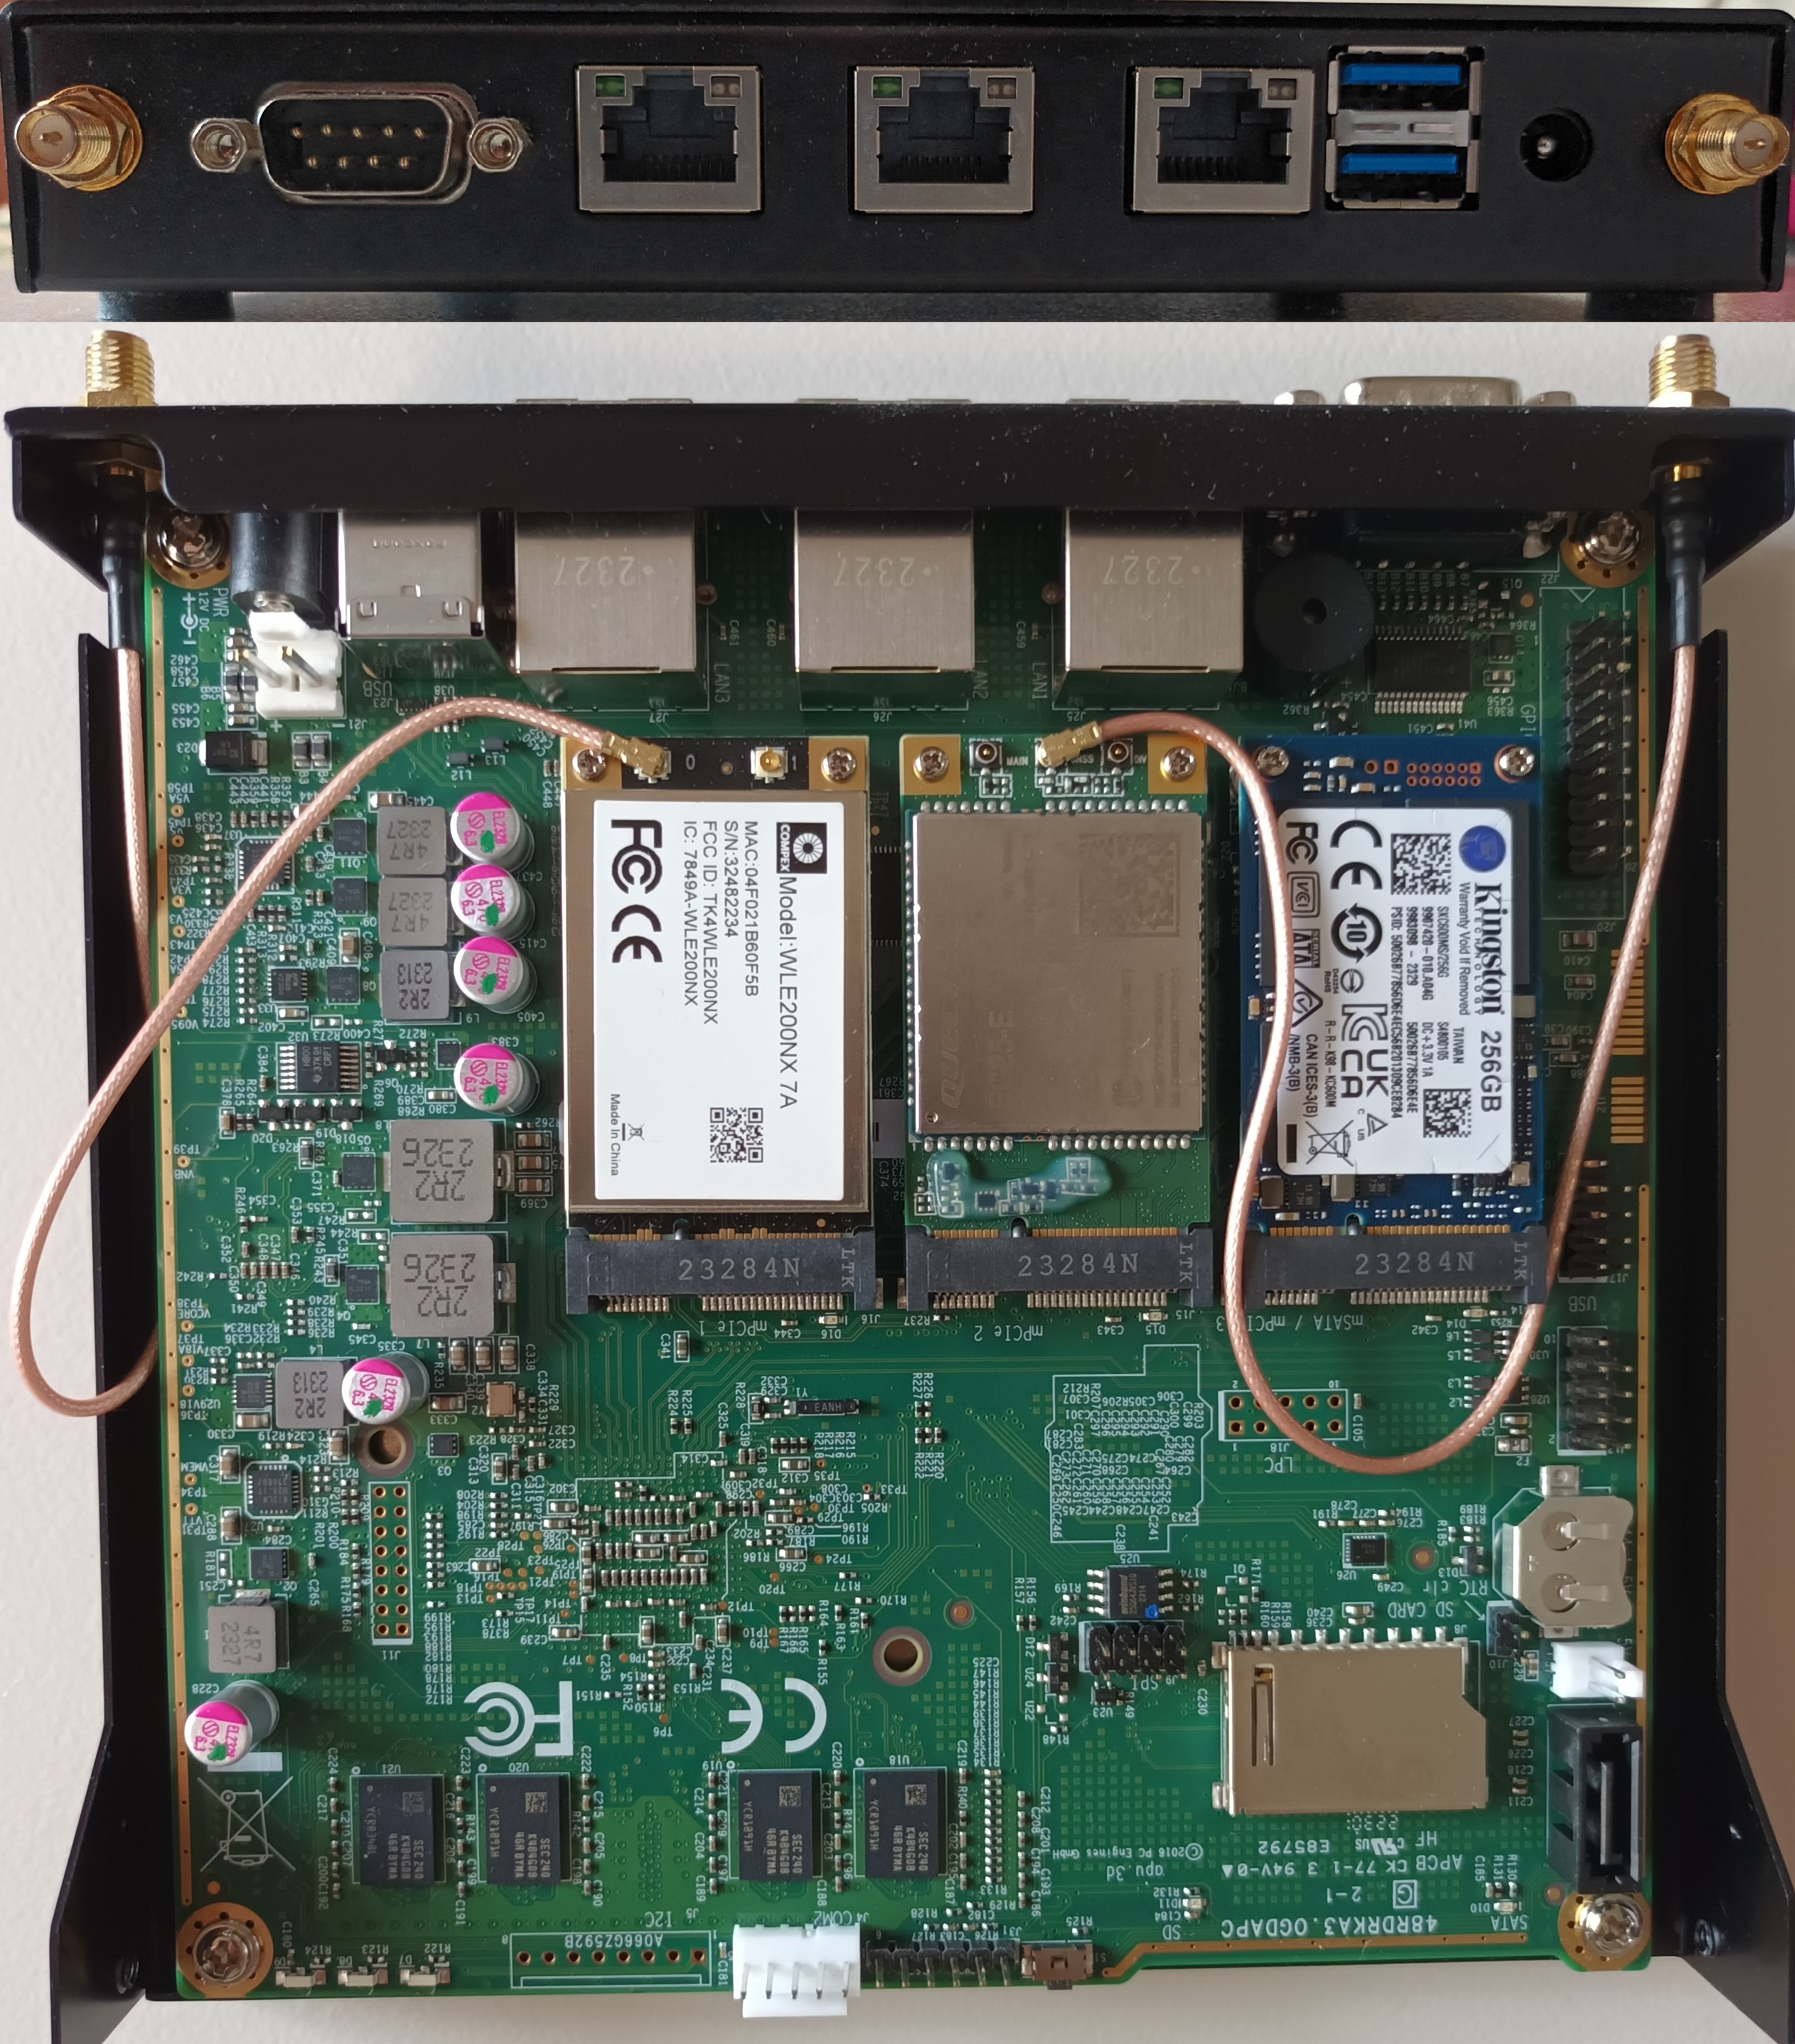
\includegraphics[width=0.5\linewidth]{Chapters/Figures/Implementation/device_1.5.jpg}}%
    \subbottom[Another sub-figure\label{fig:rightsubfig}]{%
        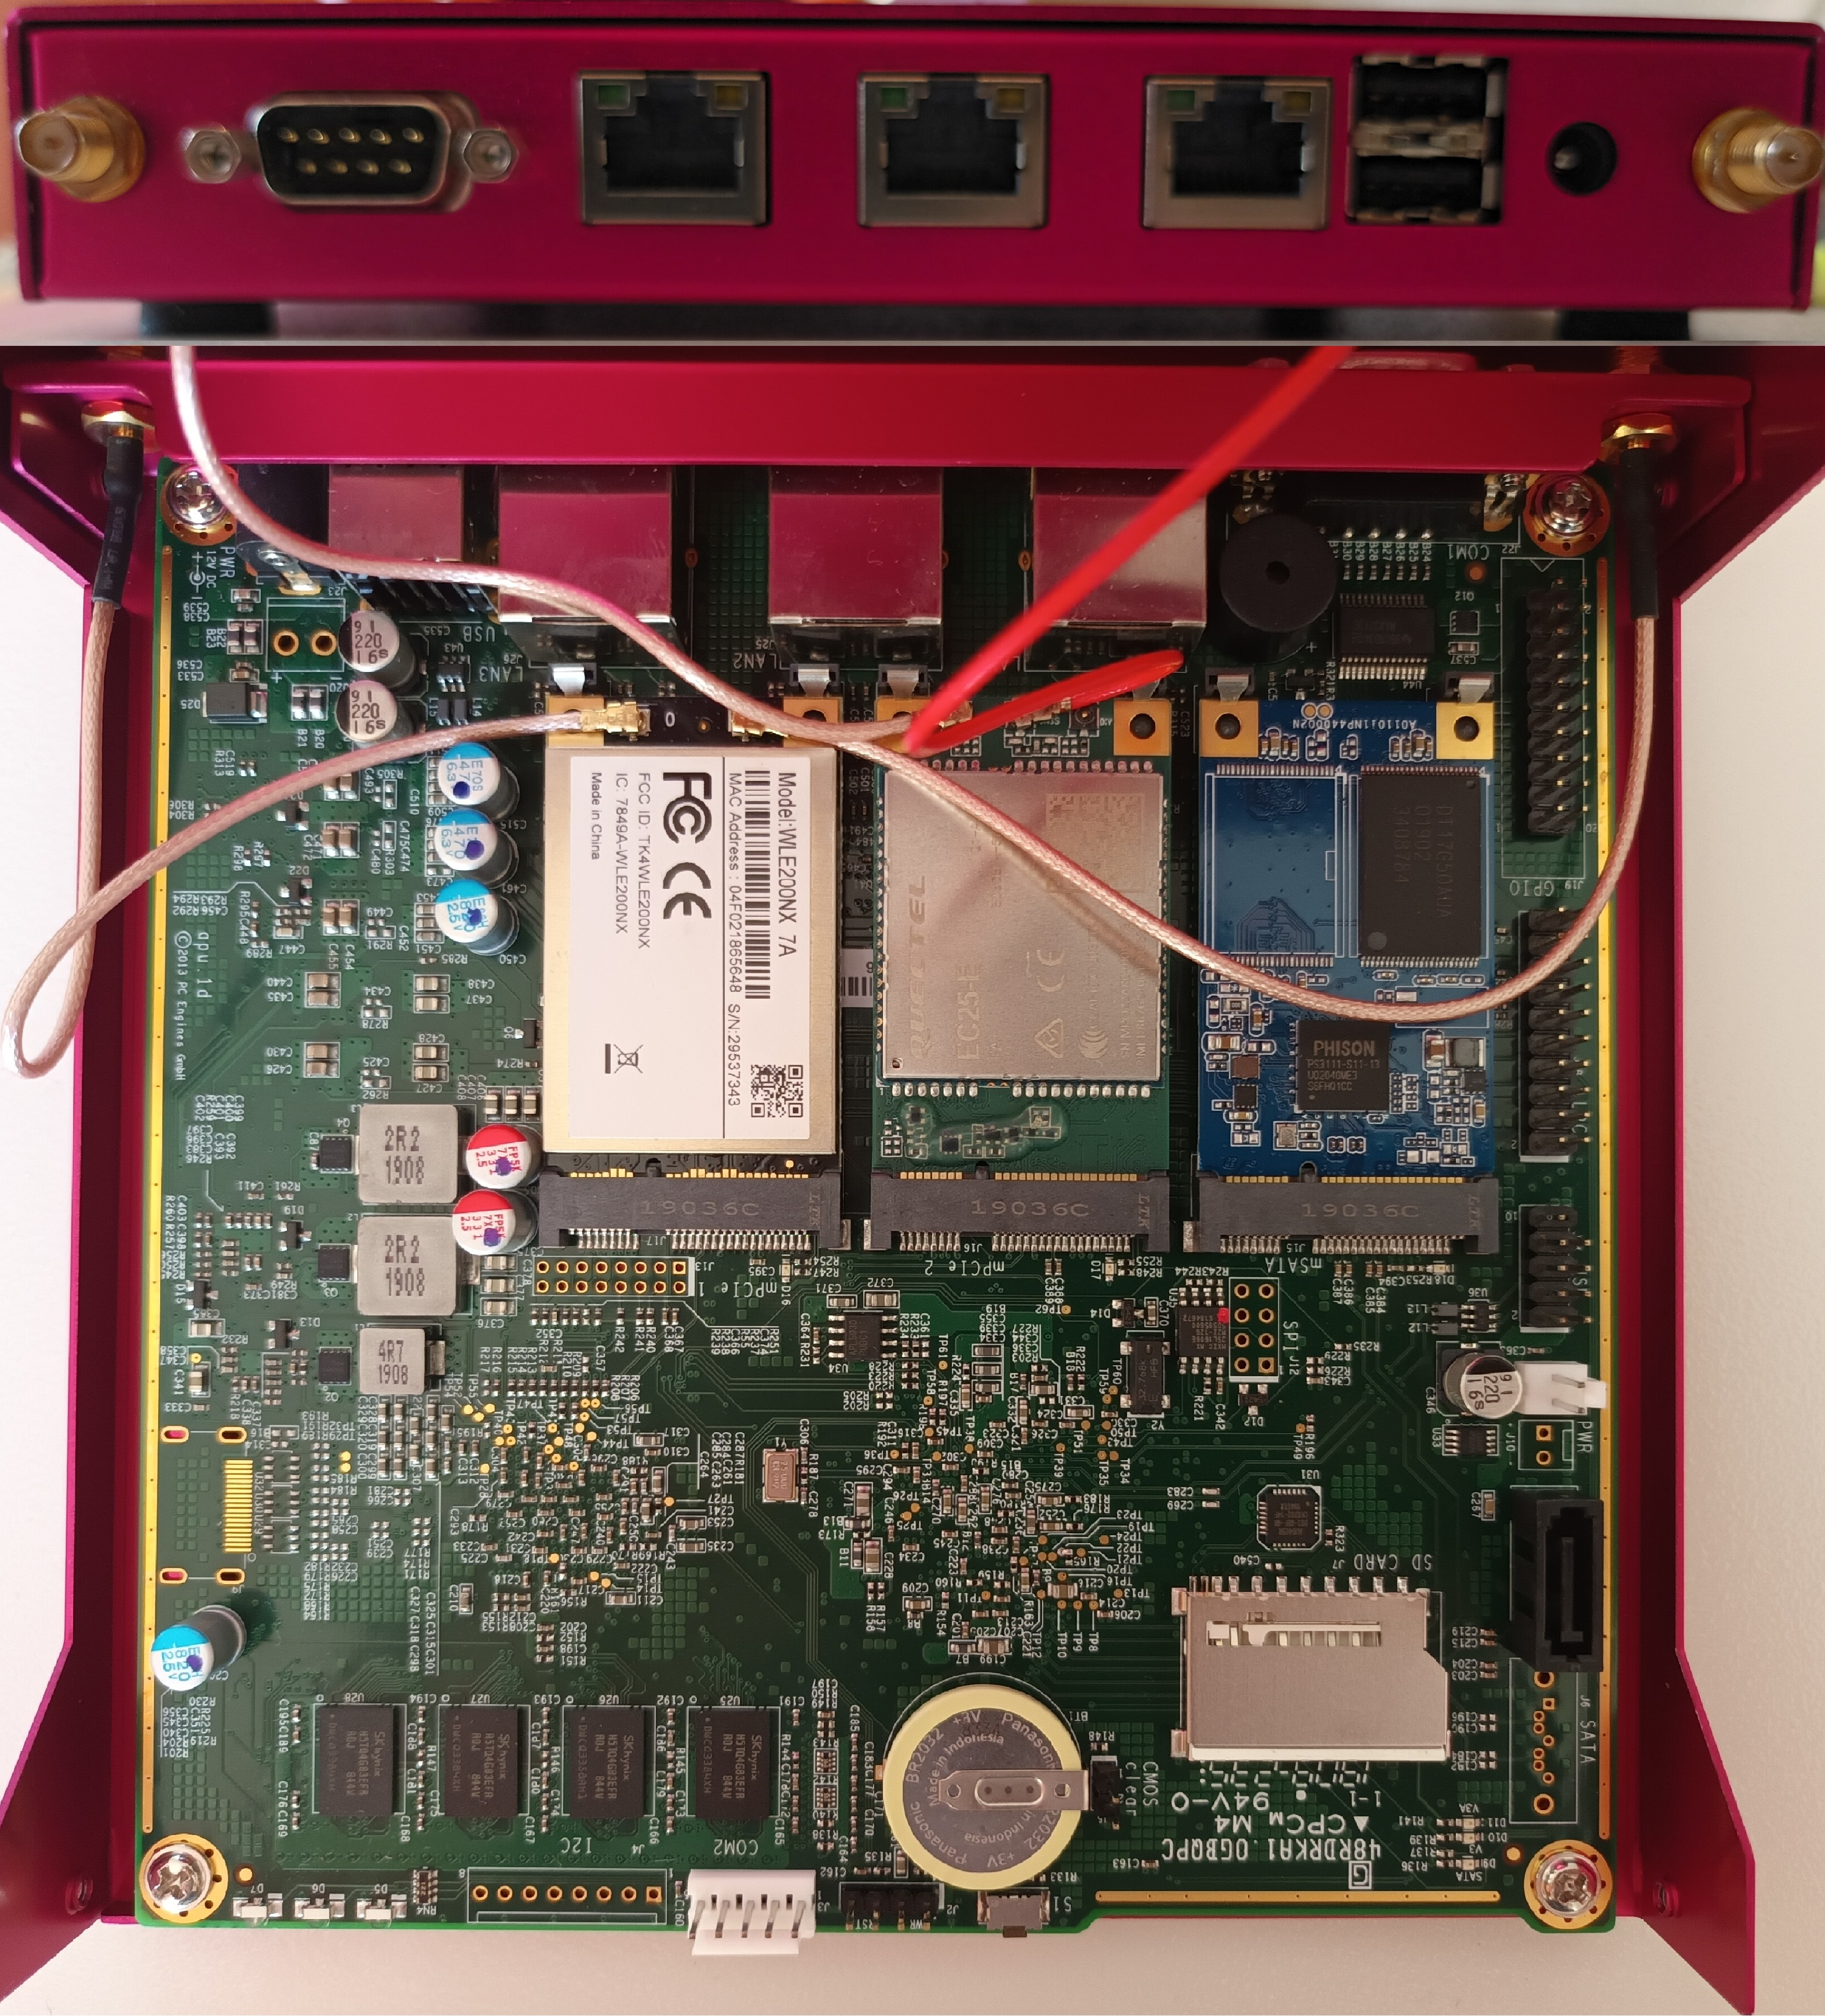
\includegraphics[width=0.5\linewidth]{Chapters/Figures/Implementation/device_1.jpg}}%
    \caption{A figure with two sub-figures!}
    \label{fig:fig2subfig}
\end{figure}
  